\section{Unitarity and Sterile Neutrinos}
While global fits assume three flavors of neutrinos, additional neutrino flavors are theoretically possible.
The number of active neutrino flavors is limited to the three known flavors from the measurements of ALEPH (see the discussion of Section~\ref{sec:neutrinos}), although such measurements implicitly only measure the number of species with a coupling to the Z boson \cite{ALEPH-3Nu}.
Additional flavors with no or very small couplings to the Z boson may be allowed \cite{Review-LightSterile}.
New neutrino flavors introduced with these properties are known as \emph{sterile neutrinos}.

\label{subsec:steriles}
\subsection{Sterile Neutrinos}
Models of sterile neutrinos assume that no weak interactions are available to the new species, leaving only interactions with the world via oscillations.
In this model, neutrinos oscillate using a 4x4 (or larger NxN) PMNS matrix \cite{Review-PMNS, GlobalSteriles-2012, GlobalSteriles-2017, Review-LightSterile}.

\begin{equation}
\begin{pmatrix} \nu_e\left(x\right) \\ 	\nu_\mu\left(x\right) \\	\nu_\tau\left(x\right) \\  \nu_s\left(x\right)\end{pmatrix} = 
U_{4x4} \begin{pmatrix} \nu_e\left(x\right) \\ 	\nu_\mu\left(x\right) \\	\nu_\tau\left(x\right) \\	\nu_s\left(x\right)\end{pmatrix} = 
\begin{pmatrix}
 U_{e 1} & U_{e 2} & U_{e 3} & U_{e 4} \\
 U_{\mu 1} & U_{\mu 2} & U_{\mu 3} & U_{\tau 4}  \\
 U_{\tau 1} & U_{\tau 2} & U_{\tau 3} & U_{\tau 4}  \\
 U_{s 1} & U_{s 2} & U_{s 3} & U_{s 4}  \\
\end{pmatrix} 	
\begin{pmatrix} \nu_1\left(x\right) \\ 	\nu_2\left(x\right) \\	\nu_3\left(x\right) \\ \nu_4\left(x\right) \end{pmatrix}
\label{eqn:4flavor_pmns}
\end{equation}

The additional terms in $U_{4x4}$ lead to new mixing angles, $\theta_{14}$, $\theta_{24}$, and $\theta_{34}$.
The new terms may be used in the standard oscillation framework introduced in Section~\ref{subsec:vacuum} extended with a fourth flavor state, ${\nu_s}$, and mass state, ${\nu_4}$.

\begin{equation}
P\left(\nu_\alpha\rightarrow\nu_\beta\right) =  \sum_i^{4} U^*_{\beta i} U_{\alpha i} \sum_j U_{\beta j} U^*_{\alpha j} e^{i \left(E_i-E_j\right) t} \ \ \ \alpha,\beta = e,\mu\tau,s
\label{eqn:sterile_pmns_probability_expanded}
\end{equation}

Unlike the three active neutrinos, sterile neutrinos cannot interact with matter, leading to a deficit in the neutrino rates from oscillations of the form ${P\left(\nu_\alpha\rightarrow\nu_s\right)}$.
The location and size of the deficit is determined by the oscillation parameters associated with the ${\nu_s}$ and ${\nu_4}$ states.
Sterile neutrinos may be indirectly observed through this deficit by studying the active neutrinos with either charged current or neutral current interactions.

\subsection{Direct Searches for Steriles}
While oscilation of the three active neutrinos preserves the total neutral current rate, sterile neutrinos do not.
This provide a unique experimental signature for sterile neutrinos.
Dedicated searches for this disappearance have been performed by MINOS \cite{MINOS-SterileNC-2011,MINOS-SterileNC-2016} and NO${\nu}$A \cite{NOvA-SterileNC} with assumptions on the new terms of the mixing matrix.
The effect of three sterile hypotheses on the MINOS data is shown in Figure~\ref{fig:minos_sterile_expectation}. 
Around 15\% of the neutral current events disappear in the three hypotheses tested by MINOS.
The results of the NO${\nu}$A search are shown in Figure~\ref{fig:sterile_limits_mu4_tau4}.

\begin{figure}[!h]%                                                                                                                                                   
        \centering
                \subfloat[MINOS NC Sterile Expectation]{
                        \label{fig:minos_sterile_expectation}
                        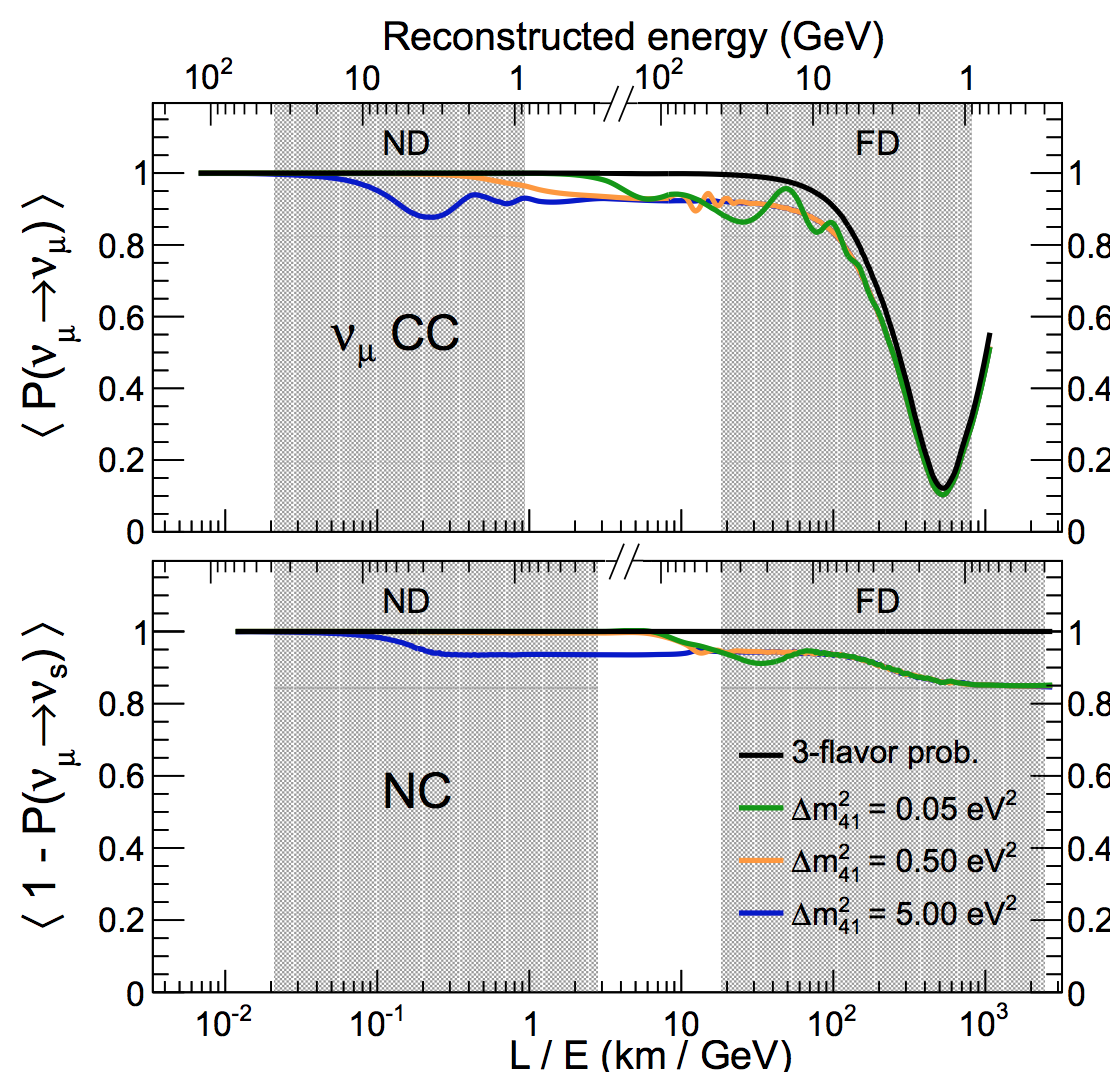
\includegraphics[width=0.4\linewidth]{minos_sterile_nc.png}}
                \subfloat[NO${\nu}$A Limits from NC Oscillations]{
                        \label{fig:sterile_limits_mu4_tau4}
                        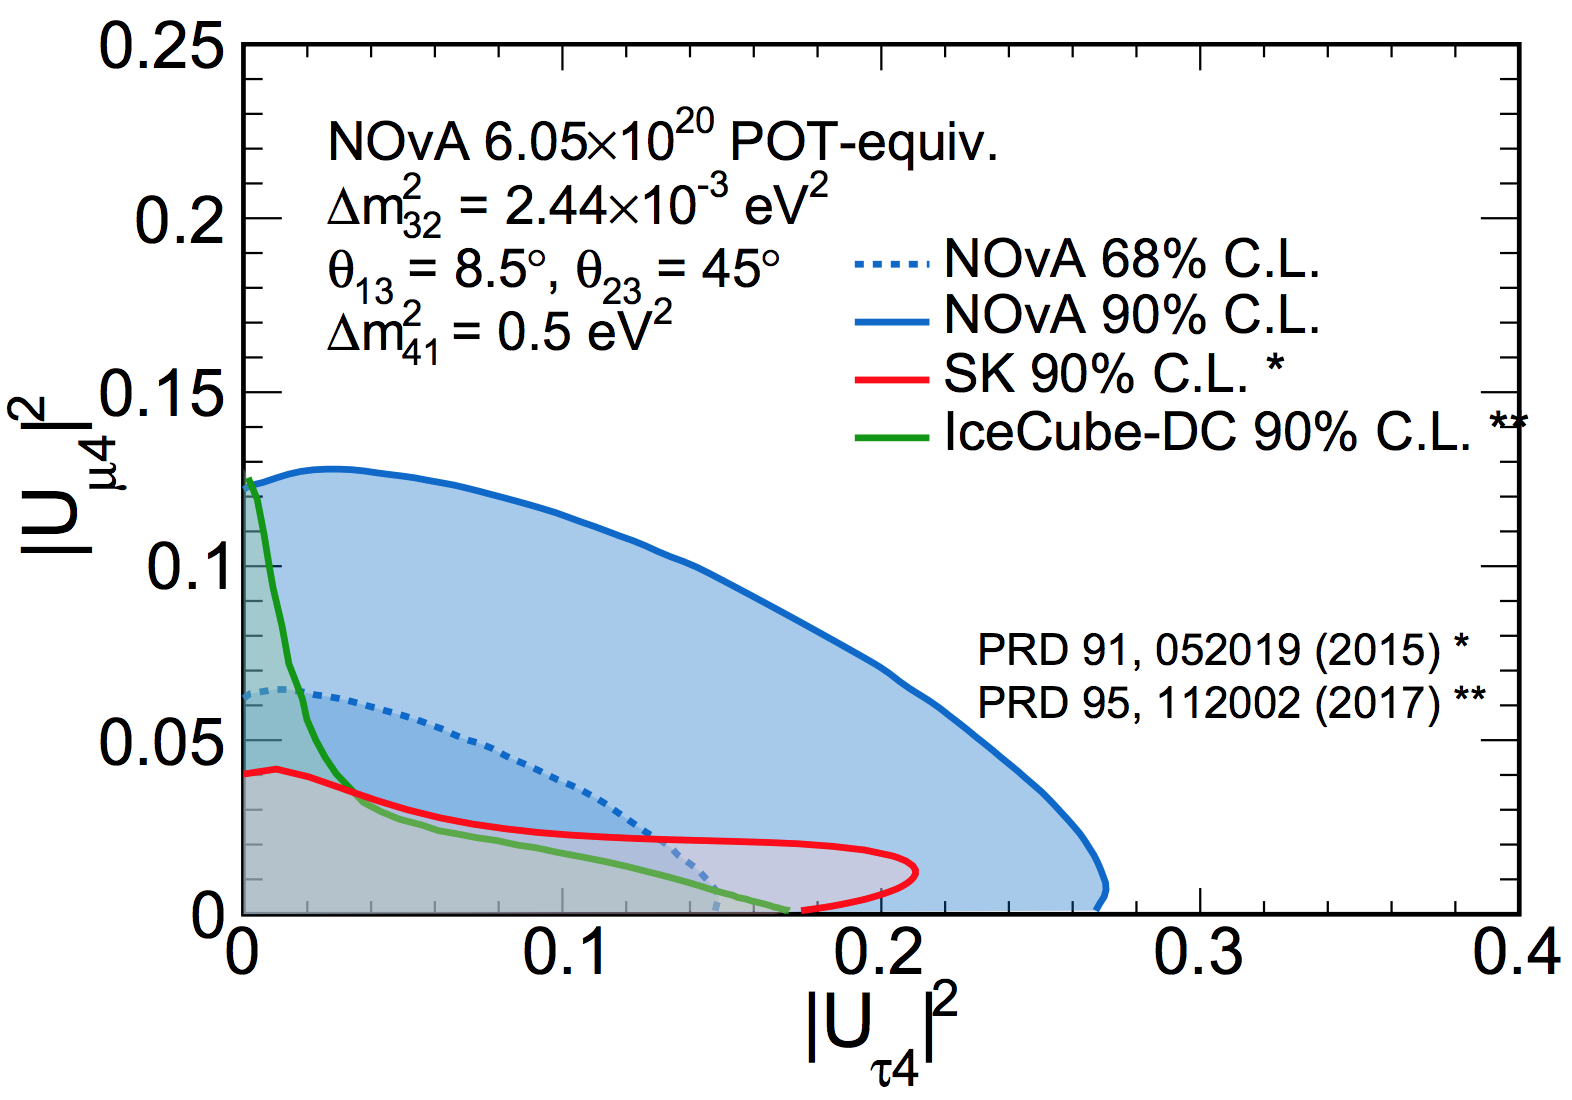
\includegraphics[width=0.4\linewidth]{nova_sterile_constraints.png}}
\caption{Expectations (a) and results (b) of searches for sterile neutrinos in the neutural current interactions. (a) Effect of three hypothetical sterile neutrinos on the measurements of the MINOS detector \cite{MINOS-SterileNC-2016}. "ND" and "FD" refer to the near and far detector of MINOS respectively. The sterile neutrinos have a small effect on the main oscillation minimum in the charged current channel, but up to 15\% of the neutral current events are lost. (b) The results of the NO${\nu}A$ search for sterile neutrinos using neutral current events. The limits are interpreted in terms of the 4x4 PMNS mixing elements in order to compare to searches with charged current interactions in Super-Kamiokande \cite{SuperK-Steriles2015} and IceCube \cite{IceCubeSterile-Andrii}. }
\end{figure}

Most experiments attempt to investigate one of the additional terms only, assuming the remainder to be negligible \cite{SuperK-Steriles2015, IceCubeSterile-Andrii, IceCubeSterile-IC86-1}. 
The results rule out large mixing between a hypothetical sterile neutrino and the three active flavors, although small mixing angles are still allowed by experiments \cite{GlobalSteriles-2017, Review-LightSterile}.

\label{subsec:steriles_unitarity}
\subsection{Indirect Searches for Steriles Using Unitarity}
Experiments need not search for direct evidence of new mixing terms, however.
The addition of a fourth generation of neutrino would have consequences for neutrino oscillation measurements performed in the 3x3 PMNS framework.
Standard 3-flavor oscillation measurements may therefore be used to place limits on sterile neutrinos.

The PMNS matrix gives the change in basis and is assumed to be unitary.
The unitary condition imposes summation rules for both the rows and colums of the matrix.

\begin{equation}
\sum_i U_{\alpha i} U_{\beta i}^* = \delta_{\alpha \beta} \;\;\;\; \alpha,\beta=e, \mu, \tau
\label{eqn:unitarity_condition_flavor}
\end{equation}
\begin{equation}
\sum_i U_{\alpha i} U_{\alpha j}^* = \delta_{ij} \;\;\;\; i,j=1,2,3
\label{eqn:unitarity_condition_mass}
\end{equation}

If the neutrino mixing matrix consists of more than the three known active neutrinos, however, these unitary relations would only hold in higher dimensions.
When projected down to the observed 3x3 PMNS matrix, non-unitarity would be observed.

Neutrino oscillation measurements are performed with the assumption of 3x3 unitarity imposed, allowing the PMNS matrix to be rewritten in terms of three mixing angles and a single phase.
The appearance and disappearance probabilities in oscillation measurements are typically written in terms of these mixing angles.
Using these mixing angles, the disappearance probability for atmospheric oscillations of $\nu_\mu \rightarrow \nu_\tau$ is given by

\begin{equation}
\begin{aligned}
P\left(\nu_\mu\rightarrow\nu_\mu\right) &{}=  1 -  \left| \sum_i U^*_{\mu i} U_{\mu i} e^{-i m_i^2 L/2E} \right|^2 \\
 						&{}= 1 - \left( cos^2 \theta_{13} sin^2 2 \theta_{23} + sin^4 \theta_{23} sin^2 2 \theta_{13} \right) sin^2 \left( \frac{\Delta m^2_{31} L}{4 E} \right) \\
 						&{}\approx 1 - sin^2 2 \theta_{23} sin^2 \left(\frac{\Delta m^2_{31} L}{4 E} \right).
\end{aligned}
\label{eqn:mu_disappearance_probability}
\end{equation}

where the final approximation has been made due to the small value of $\theta_{13}$.
The atmospheric appearance probability, $\nu_\mu \rightarrow \nu_\mu$, is given by

\begin{equation}
\begin{aligned}
P\left(\nu_\mu\rightarrow\nu_\tau\right) {}= &  \left| \sum_i U^*_{\mu i} U_{\tau i} e^{-i m_i^2 L/2E} \right|^2 \\
 						&{}= \left( cos^2 \theta_{13} sin^2 2 \theta_{23} \right) sin^2 \left( \frac{\Delta m^2_{31} L}{4 E} \right) \\
						&{}\approx sin^2 2 \theta_{23} sin^2 \left(\frac{\Delta m^2_{31} L}{4 E} \right).
\end{aligned}
\label{eqn:tau_appearance_probability}
\end{equation}

The form of the oscillation probabilities for appearance and disappearance are very similar when written in terms of the mixing angles.
However, the appearance and appearance probabilities in neutrino oscillation measurements depend on different elements of PMNS mixing matrix.
Because of the difference in the elements probed, appearance and disappearance measurements may be interpreted to give limits on the fundamental elements of the mixing matrix without imposing unitary.

This method of searching for sterile neutrinos may be applied to global fits, reinterpreting standard oscillation measurements to place limits on the size of any non-unitarity.
Using the unitarity conditions of Equation~\ref{eqn:unitarity_condition_flavor} and \ref{eqn:unitarity_condition_mass}, limits on the size of non-untarity have been calculated\cite{Parke-Unitarity}.
Experimental constraints from a number of experiments (see reference 26 of \cite{Parke-Unitarity}) were used to evaluate the best-fit mixing matrix.
The unitarity constraints were tested by looking at the potential deviation of each row or column

\begin{equation}
	\Delta U_{\alpha} = 1 - \left( \left| U_{\alpha 1} \right|^2 +\left| U_{\alpha 2} \right|^2 +\left| U_{\alpha 3} \right|^2 \right) \;\;\;\; \alpha=e, \mu, \tau
\label{eqn:unitarity_flavor_test}
\end{equation}
or 
\begin{equation}
	\Delta U_{i} = 1 - \left( \left| U_{\alpha i} \right|^2 + \left| U_{\beta i} \right|^2 + \left| U_{\delta i} \right|^2 \right) \;\;\;\; i=1, 2, 3
\label{eqn:unitarity_mass_test}
\end{equation}

The results are shown in \ref{fig:unitarity_norms}.
The contraints on unitarity of the 3x3 mixing matrix are strongest in the muon and electron sector, with constraints nearly an order of magnitude stronger than that observed in the tau sector.
This is a result of limited measurements directly involving $\nu_\tau$ oscillations.

\begin{figure}[!h]%
	\centering
	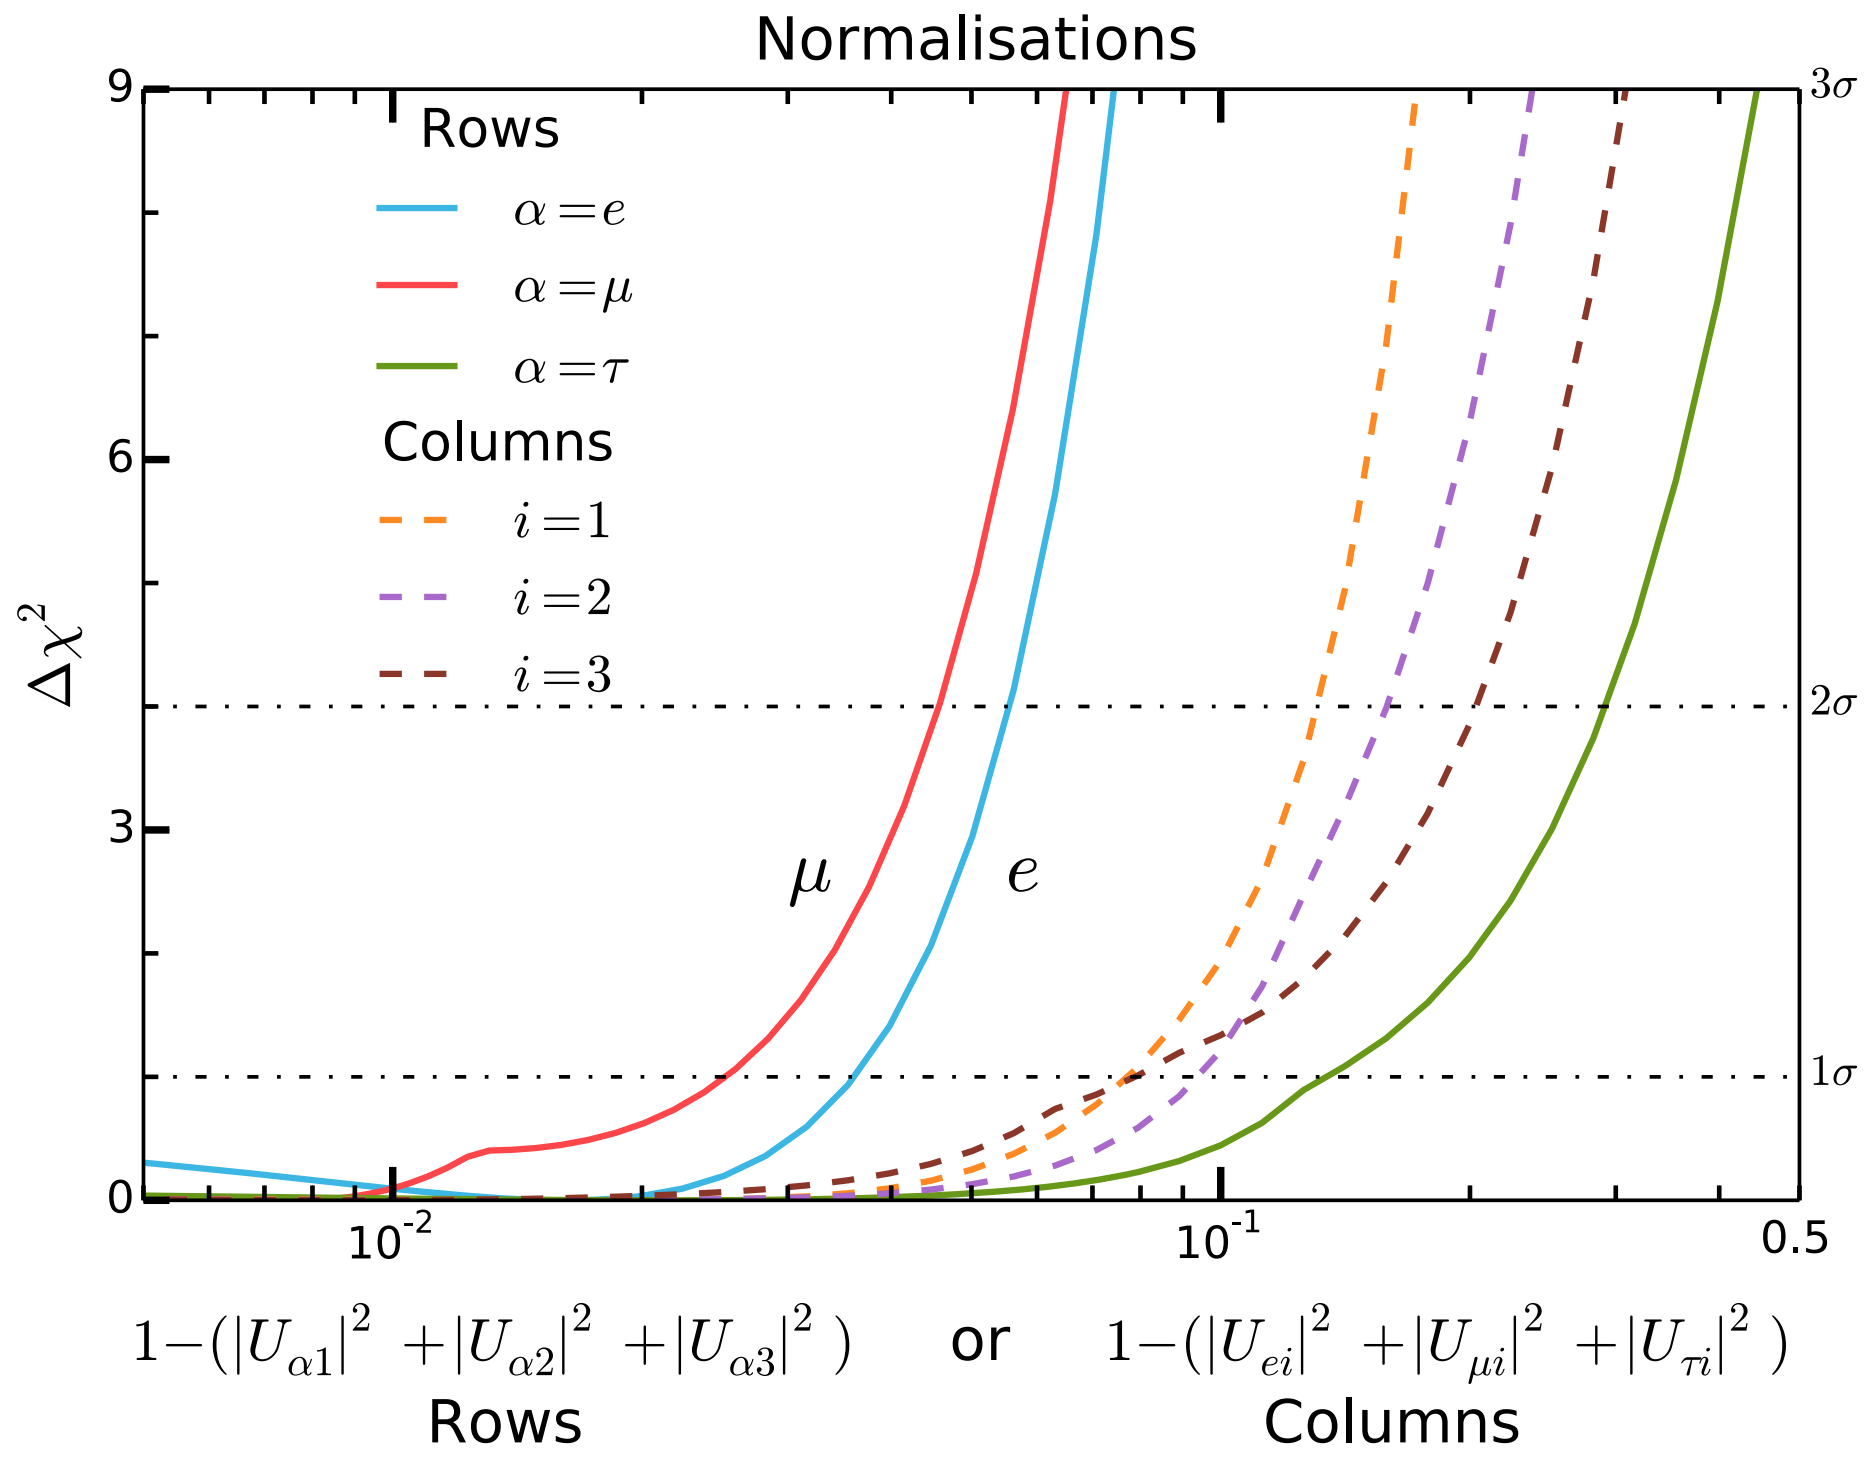
\includegraphics[width=0.7\linewidth]{unitarity_norms.png}%
	\caption{The results of the tests using \ref{eqn:unitarity_flavor_test} (solid) and \ref{eqn:unitarity_mass_test} (dotted). A smaller value on the x-axis indicates a tighter constraint on observed unitarity of the 3x3 mixing matrix. Tests involving only muon or electron flavors show significantly tighter constraints than those including the tau flavor.	Image taken from \cite{Parke-Unitarity}}
	\label{fig:unitarity_norms}
\end{figure}

\begin{landscape}
\begin{figure}[!h]%
	\centering
	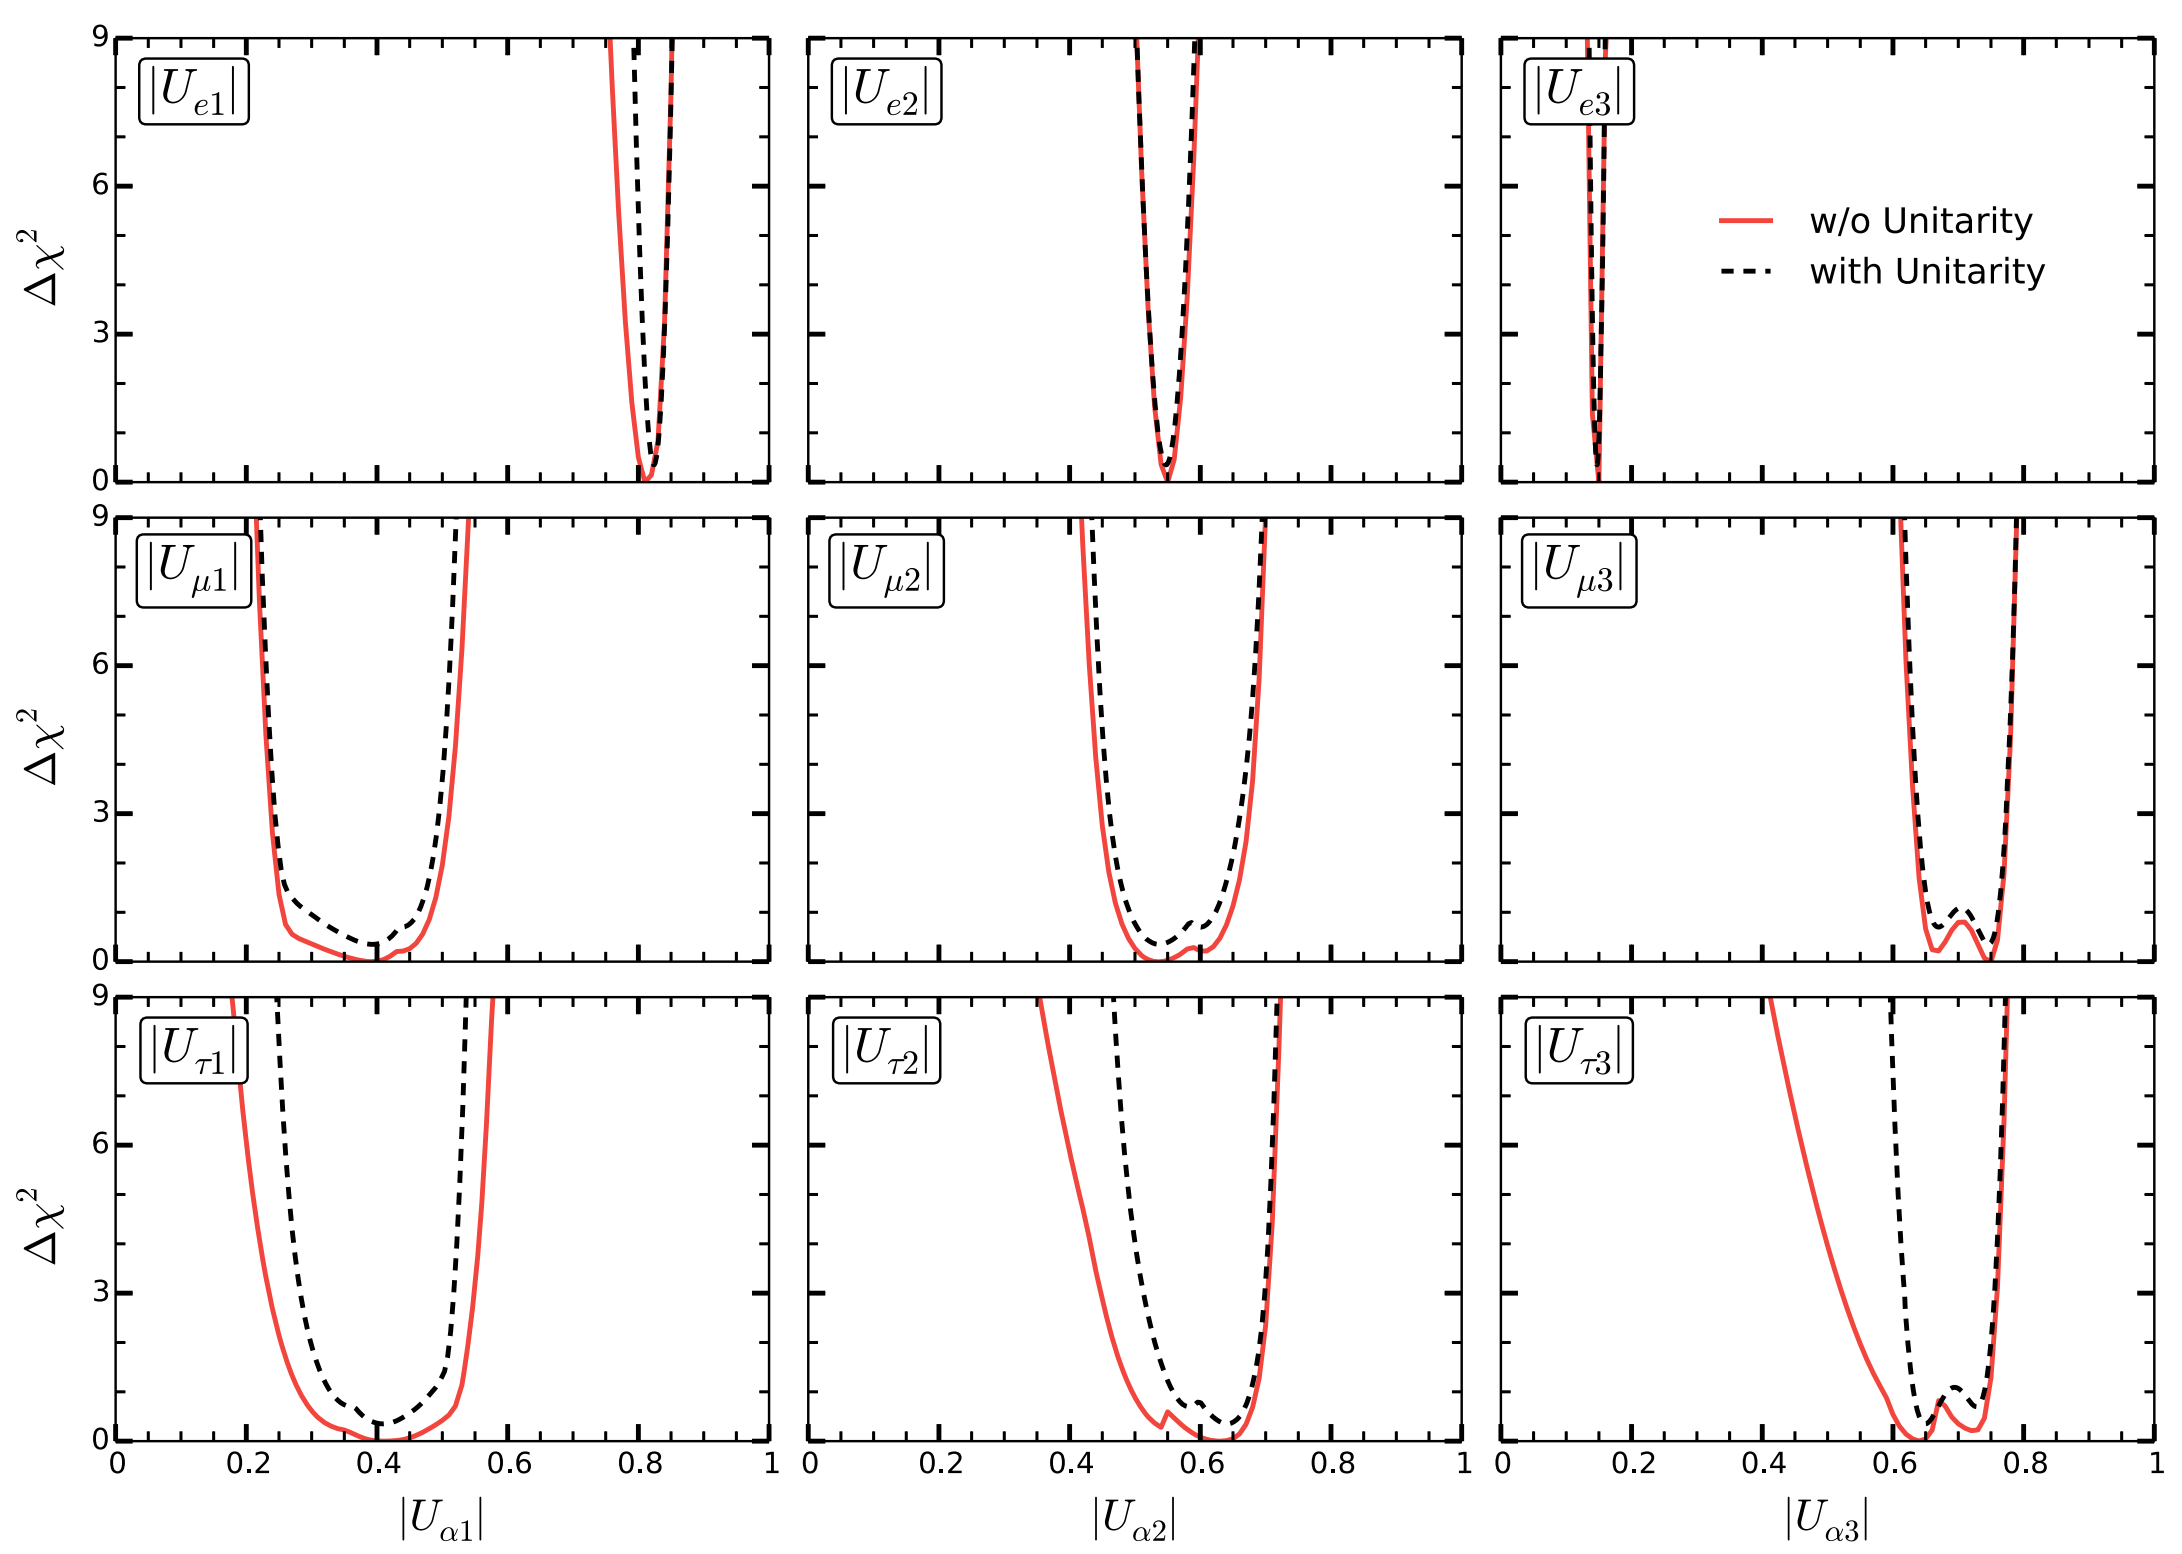
\includegraphics[width=0.8\linewidth]{pmns_unitarity.png}%
	\caption{The constraints from a global fit to neutrino oscillation data\cite{Parke-Unitarity} with an assumption of unitarity (black dotted) or no assumption of unitarity (red solid). The first two rows show little change from the unitarity assumption, indicating strong constraints from direct measurements. The elements of the third row, related to the $\nu_\tau$, show much larger changes, indicating that constraints are obtained from indirect oscillation measurements. }
	\label{fig:pmns_unitarity}
\end{figure}
\end{landscape}

When the individual limits for each element of the 3x3 PMNS matrix are checked, it is the tau sector that shows the largest uncertainties.
Measurements of $\nu_\tau$ oscillations therefore can provide valuable information on unitarity in the neutrino sector, leading to indirect constaints on sterile neutrino hypotheses.

